Traumatic Brain Injury (TBI) occurs from an impact to the head resulting in an injury to the brain, commonly caused by road traffic accidents and falls \cite{Langlois2006}. The severity of the injury sustained to the brain can range from superficial swelling to oedema and haematomas, with higher severity of the TBI resulting in a higher mortality rate as shown in Table~\ref{table:severity of TBI}. Even if the injury does not result in death, TBI can lead to long term disability and cognitive problems \cite{WorldHealthOrganisation2006}. Approximately 2.5 million people visited the hospital for TBI related symptoms in the US during 2013, of which 56,000 result in death \cite{Taylor2017}. The prevalence of this injury incurs an estimated \$60 billion cost annually to society to cover medical costs and lost productivity \cite{Finkelstein2009}. 

Primary TBI is the damage sustained from the initial impact, whereas secondary TBI occurs from the cascade of biochemical processes following from primary TBI, resulting in damage to the tissue surrounding the primary injury site \cite{Norton2008}. Secondary TBI tends to occur after a delayed period of time in about 30\%-40\% of people who have suffered primary TBI, however whether it occurs is unpredictable and unpreventable \cite{Pagkalos2017}. Secondary effects, such as oedema, hypoxia and ischemia, can lead to neural degeneration and irreversible damage which can cause severe disability or be fatal \cite{Murthy2005}. Hence, it is crucial to diagnose secondary TBI as soon as possible and provide appropriate medication to treat and minimise the damage.

\begin{table}[H]
\centering
\begin{tabular}{||c c||} 
 \hline
 Severity of TBI & Mortality (\%) \\ [0.5ex] 
 \hline\hline
 Mild & \textless 1 \\ 
 Moderate & 2-5 \\
 Severe & 20-50 \\
 \hline
\end{tabular}
\caption{Severity of TBI affecting mortality rates \cite{WorldHealthOrganisation2006}}
\label{table:severity of TBI}
\end{table}

Common methods used to diagnose secondary TBI rely on qualitative analysis. An example is the Glasgow Coma Scale which assesses ocular, verbal and motor responses and assigns a score out of 15. This is then accompanied with a neuroimaging method such as a CT scan \cite{WorldHealthOrganisation2006}. The main disadvantage of these methods is that they are subjective, and it is difficult to identify mild symptoms of TBI which are displayed subtly as non-specific symptoms \cite{Bettermann2012}. Furthermore, these methods only capture information at a specific period in time meaning that if symptoms occur, they will be unobserved until the next appointment. 

Early diagnosis is crucial for the best recovery, and to do so, there is a need to continuously monitor the patient and receive quantitative data for accurate diagnosis. The Boutelle Research Group have been looking into utilising brain signals that are associated with TBI. From the primary injury site, spreading depolarisation (SD) waves propagate into surrounding brain tissue and cause secondary damage. The cells in the injury sites have a high energy demand in order to repolarise the membrane potential, hence the glucose concentration in the extracellular fluid transiently decreases by approximately 18-93$\mu M$. The cells tend to undergo anaerobic respiration, so the extracellular lactate concentration transiently increase by 5-100$\mu M$ \cite{D.2010}. Glucose and lactate have been declared by the International Microdialysis Collaborative Group as the most clinically useful signals for the prognosis of TBI \cite{Hutchinson2015}. Furthermore, during the same transient period, the potassium ion concentration increases \cite{Rogers2017} as shown in Figure~\ref{fig: SD}.

\begin{figure}[t]
\centering
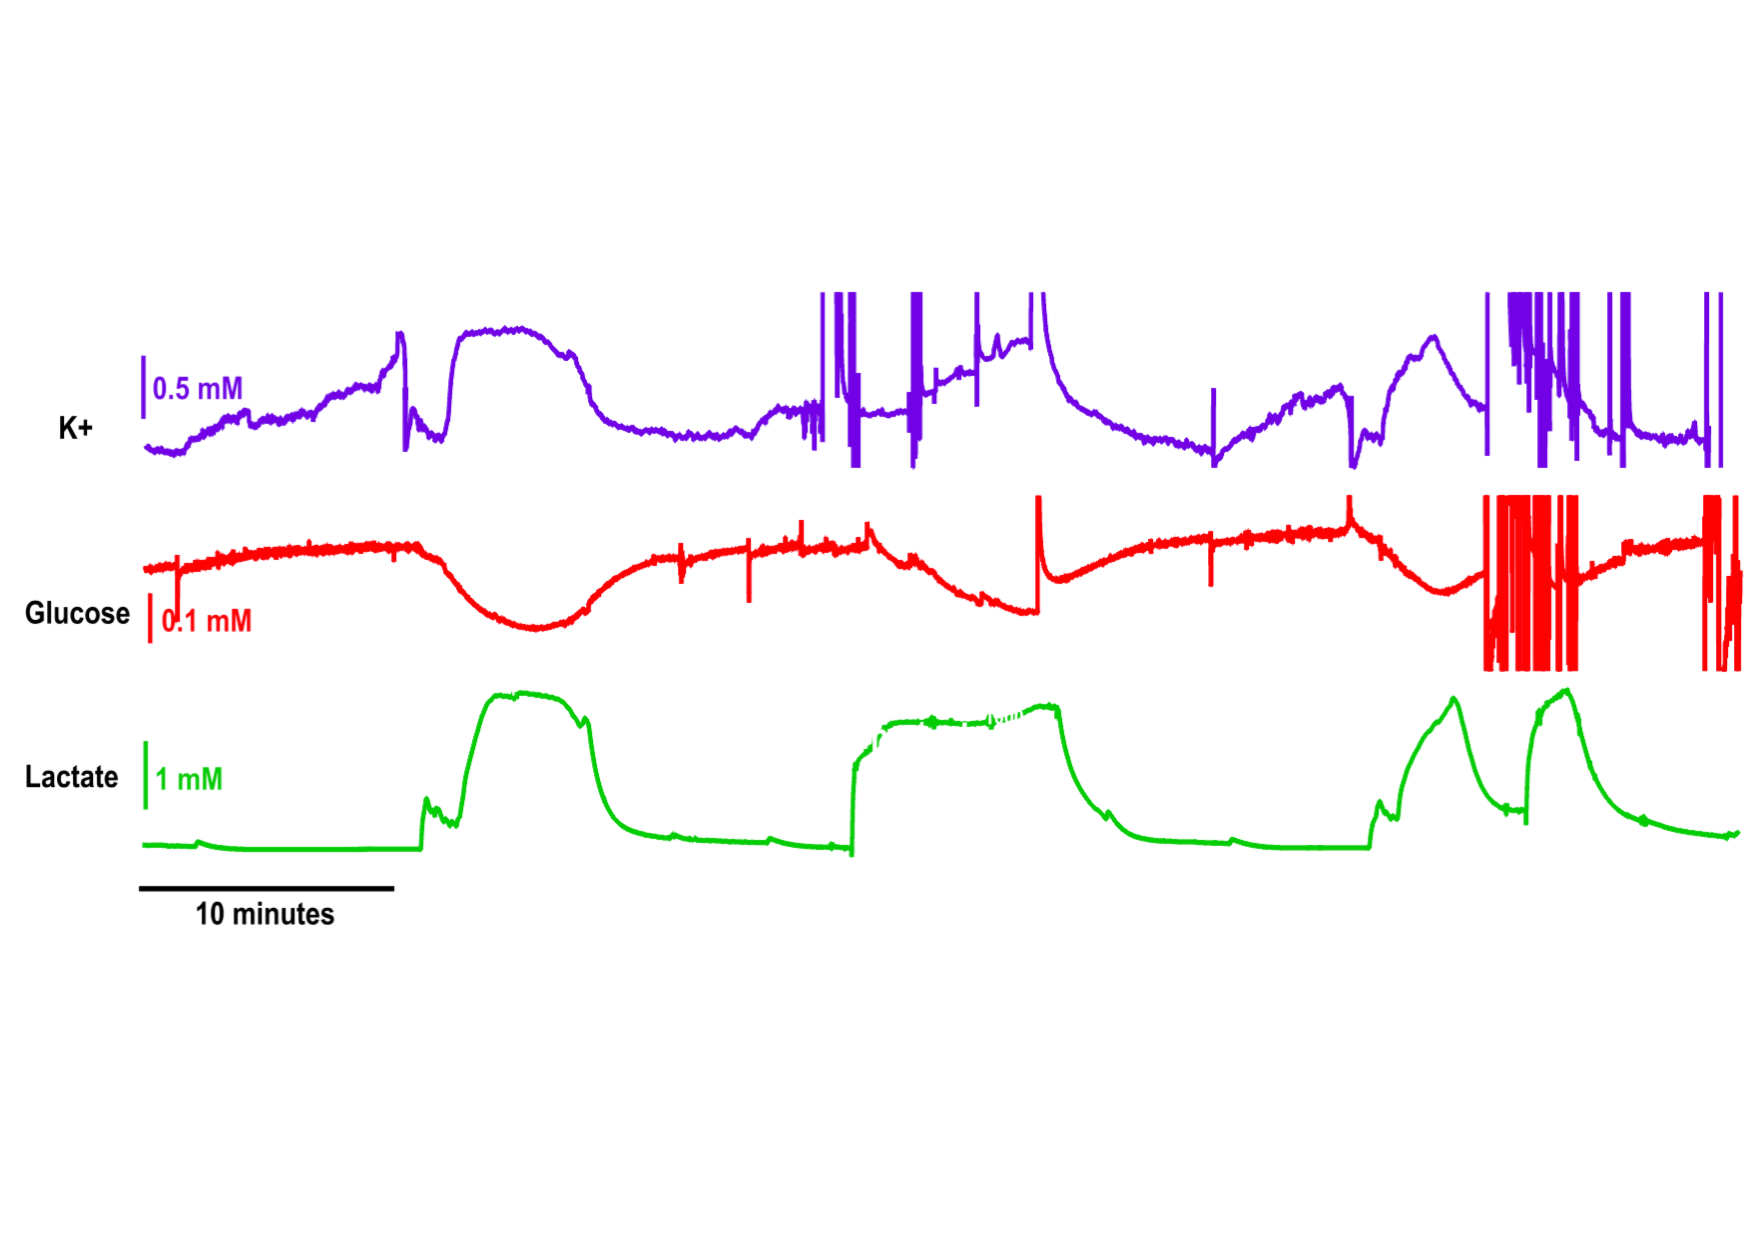
\includegraphics[trim={0cm 5cm 0.5cm  5cm}, clip, width=1\textwidth]{./figures/conc.pdf}
\captionsetup{justification=centering}
\caption{Biochemical changes during an SD occurence at 10 minutes. K+ and lactate show an increase in concentration whilst glucose shows a decrease in concentration \cite{Rogers2017}. Measurements obtained from microdialysis.}
\label{fig: SD}
\end{figure}

The research group have developed the LENBIC, and ASIC (application specific integrated chip) which can measure these three electrochemical signals of interest using the microdialysis system inserted into the brain \cite{Pagkalos2017}. It contains amperometric channels for the detection of glucose and lactate, and potentiometric channels for the detection of potassium ions from the microdialysis system it is connected to. However, the LENBIC is a wired system, so its limitations include requiring an orifice for the wires to exit the body, the patient's movement is restricted, the wires may break, and the wires may introduce noise \cite{Ferguson2011}. Therefore, a wireless transmission system is more desirable to communicate the electrochemical data. 

\textbf{DOUBLE CHECK WITH MICHELLE ABOUT THIS}
Furthermore, data is extracted from the microdialysis system at the end of experimentation and is later analysed manually by someone who is trained to identify when an SD has occurred. This prevents diagnosis from occurring sooner at the time of the SD. There is a need for the data to be received and analysed in real time to ensure early diagnosis. 

This project aims to develop a wireless communication system between the microdialysis system and an iOS application. Information from the three electrochemical sensors will be received simultaneously in an iPad application in real time. The app must be user friendly and be of high quality as it aims to be used by a clinician to monitor the state of the patient. It is important that the signals are transmitted and displayed accurately so suitable processing methods need to be implemented. 

